\documentclass[a4paper,10pt,uplatex,dvipdfmx]{jsarticle}


% 数式
\usepackage{amsmath,amsfonts}
\usepackage{bm}
% 画像
\usepackage[dvipdfmx]{graphicx}
\usepackage{here}
% program
\usepackage{color}
\usepackage{listings, jlisting}
\input{listings-glsl.prf}
% 枠付き
\usepackage{ascmac}

\lstset{
 language={C++},%言語の指定
%  backgroundcolor={\color[gray]{.85}},%背景色と透過度
 basicstyle={\ttfamily},%書体の指定
 identifierstyle={\small\color[rgb]{0.8,0.5,0}},%キーワードでない文字の書体
 commentstyle={\small\itshape\color[rgb]{0,0.3,0}},%注釈の書体
 keywordstyle={\small\bfseries\color[rgb]{0,0.5,1}},%キーワード(int, ifなど)の書体指定
 ndkeywordstyle={\small},%
 stringstyle={\small\ttfamily\color[rgb]{1,0.5,0}},%文字列
 frame={tb},%枠縁(leftline,topline,bottomline,lines,trBL,shadowbox, single)
 breaklines=true,%折り返し(自動改行)
 breakindent = 10pt,  %自動改行後のインデント量(デフォルトでは20[pt])	
 columns=[l]{fullflexible},%
 numbers=left,%行番号表示
 xrightmargin=0zw,%
 xleftmargin=3zw,%
 numberstyle={\scriptsize},%行番号の書体指定
 stepnumber=1,
 numbersep=1zw,%
 lineskip=-0.5ex%
}
\renewcommand{\lstlistingname}{Code} % キャプション名の指定

\begin{document}
\title{アドバンストCG\\ \huge 第6回レポート}
\author{学籍番号:201811411\\ 所属:情報学群情報メディア創成学類\\ 氏名:加藤虎之介}
\date{\today}
\maketitle

\section{実行環境}
\subsection{実行に用いたOS}
macOS Big Sur ver11.3.1

\subsection{プログラム起動時に表示される情報}
\begin{screen}
	OpenGL version: 2.1 ATI-4.4.17\\
	GLSL version: 1.20\\
	Vendor: ATI Technologies Inc.\\
	Renderer: AMD Radeon Pro 5300M OpenGL Engine
\end{screen}

\section{課題A}
\subsection{修正したソースコード}

\subsubsection{Stretching Constraintの実装}
\begin{lstlisting}[caption=pbd.cppのprojectStretchingConstraint関数]
	void ElasticPBD::projectStretchingConstraint(float ks)
	{
		if (m_iNumEdge <= 1)
			return;
	
		for (int i = 0; i < m_iNumEdge; ++i)
		{
			// 四面体を使うときの内部エッジかどうかの判定&内部エッジを使うかどうかのフラグチェック
			if (m_vInEdge[i] && !m_bUseInEdge)
				continue;
	
			// エッジ情報の取得とエッジ両端の頂点番号および質量の取得(固定点の質量は大きくする)
			const rxEdge &e = m_poly.edges[i];
			int v1 = e.v[0];
			int v2 = e.v[1];
			float m1 = m_vFix[v1] ? 30.0f * m_vMass[v1] : m_vMass[v1];
			float m2 = m_vFix[v2] ? 30.0f * m_vMass[v2] : m_vMass[v2];
			if (m1 < glm::epsilon<float>() || m2 < glm::epsilon<float>())
				continue;
	
			// 2頂点の位置ベクトル
			glm::vec3 p1 = m_vNewPos[v1];
			glm::vec3 p2 = m_vNewPos[v2];
	
			// 計算点間の元の長さ(制約条件)
			float d = m_vLengths[i];
	
			// TODO:重力等を考慮した後の2頂点座標(スライド中のp')はp1=m_vNewPos[v1],p2=m_vNewPos[v2]で得られるので,
			//      これらから制約を満たすような位置修正量dp1,dp2を求めて,m_vNewPos[v1],m_vNewPos[v2]に足し合わせる.
			//      ◎エッジの長さによってはゼロ割が発生することがある.エラーチェックを忘れずに!
			glm::vec3 dp1, dp2;
	
			// ----課題ここから----
			// 重みの計算
			float w1 = 1.0f / m1;
			float w2 = 1.0f / m2;
	
			// p1-p2ベクトルの長さ
			float vecLength = glm::length(p1 - p2);
			// エッジの長さが閾値よりも小さい場合はスキップする。(ゼロ割り対策)
			if (vecLength < glm::epsilon<float>())
				continue;
	
			dp1 = (-w1 / (w1 + w2)) * (vecLength - d) * (p1 - p2) / vecLength;
			dp2 = (w2 / (w1 + w2)) * (vecLength - d) * (p1 - p2) / vecLength;
	
			// ----課題ここまで----
	
			// 頂点位置を修正
			if (!m_vFix[v1])
				m_vNewPos[v1] += ks * dp1;
			if (!m_vFix[v2])
				m_vNewPos[v2] += ks * dp2;
		}
	}
\end{lstlisting}

\subsubsection{Bending Constraintの実装}
\begin{lstlisting}[caption=pbd.cppのprojectBendingConstraint関数]
	void ElasticPBD::projectBendingConstraint(float ks)
	{
		if (m_iNumTris <= 1 || m_iNumEdge <= 0 || m_vBends.empty())
			return;
	
		for (int i = 0; i < m_iNumEdge; i++)
		{
			// 2つのポリゴンに挟まれたエッジ情報の取得
			const rxEdge &e = m_poly.edges[i];
			if (e.f.size() < 2)
				continue; // このエッジを含むポリゴン数が1なら処理をスキップ
	
			// 2つの三角形を構成する4頂点のインデックスを抽出
			set<int>::iterator itr = e.f.begin();
			const rxFace &f1 = m_poly.faces[*itr];
			itr++;
			const rxFace &f2 = m_poly.faces[*itr];
			int v1 = e.v[0], v2 = e.v[1], v3, v4;
			for (int j = 0; j < 3; ++j)
			{
				if (f2[j] != v1 && f2[j] != v2)
					v4 = f2[j];
				if (f1[j] != v1 && f1[j] != v2)
					v3 = f1[j];
			}
			float m1 = m_vFix[v1] ? 30.0f * m_vMass[v1] : m_vMass[v1];
			float m2 = m_vFix[v2] ? 30.0f * m_vMass[v2] : m_vMass[v2];
			float m3 = m_vFix[v3] ? 30.0f * m_vMass[v3] : m_vMass[v3];
			float m4 = m_vFix[v4] ? 30.0f * m_vMass[v4] : m_vMass[v4];
			if (m1 < glm::epsilon<float>() || m2 < glm::epsilon<float>() || m3 < glm::epsilon<float>() || m4 < glm::epsilon<float>())
				continue;
	
			// 4頂点の位置ベクトル(p2-p4はp1に対する相対位置ベクトル) -> スライドp36の^(ハット)付きのp2-p4の方
			glm::vec3 p1 = m_vNewPos[v1];
			glm::vec3 p2 = m_vNewPos[v2] - p1;
			glm::vec3 p3 = m_vNewPos[v3] - p1;
			glm::vec3 p4 = m_vNewPos[v4] - p1;
	
			// 2面間の初期角度
			float phi0 = m_vBends[i];
	
			// TODO:エッジを挟んだ4頂点座標p1,p2,p3,p4からbending constraintを満たす位置修正量dp1~dp4を求め,
			//      m_vNewPos[v1]~m_vNewPos[v4]に足し合わせる.
			//		・↑で定義しているp1~p4で,p2~p4はp1に対する相対座標(スライドp36の^(ハット)付きのp2-p4の方)にしてあるので注意
			//		・三角形ポリゴン間の角度の初期値φ0はm_vBends[i]で得られる(↑で変数phi0に代入済み)
			//      ◎ベクトルの大きさで割るという式が多いが,メッシュの変形によってはゼロ割が発生することがある.エラーチェックを忘れずに!
			//		◎スライドp36のdを計算するときに,-1~1の範囲にあるかをちゃんとチェックして,範囲外ならクランプするように!
			//      - 授業スライドに合わせるためにp1~p4など配列を使わずに書いている.
			//		  配列を使って書き換えても構わないが添え字の違い(配列は0から始まる)に注意.
			glm::vec3 dp1(0.0f), dp2(0.0f), dp3(0.0f), dp4(0.0f);
	
			// ----課題ここから----
			// n1, n2の正規化前のベクトルを_n1, _n2とする。
			auto _n1 = glm::cross(p2, p3);
			auto _n2 = glm::cross(p2, p4);
			// _n1, _n2の長さ
			float _n1Length = glm::length(_n1);
			float _n2Length = glm::length(_n2);
			// _n1, _n2の大きさによってゼロ割が発生しないか確認。
			if (_n1Length < glm::epsilon<float>() || _n2Length < glm::epsilon<float>())
				continue;
	
			// n1, n2を計算
			auto n1 = glm::normalize(_n1);
			auto n2 = glm::normalize(_n2);
	
			// dを計算
			float d = min(max(glm::dot(n1, n2), -1.0f), 1.0f);
	
			// q1~q4
			auto q3 = (glm::cross(p2, n2) + glm::cross(n1, p2) * d) / _n1Length;
			auto q4 = (glm::cross(p2, n1) + glm::cross(n2, p2) * d) / _n2Length;
			auto q2 = -(glm::cross(p3, n2) + glm::cross(n1, p3) * d) / _n1Length - (glm::cross(p4, n1) + glm::cross(n2, p4) * d) / _n2Length;
			auto q1 = -q2 - q3 - q4;
	
			// 重み
			float w1 = 1.0f / m1;
			float w2 = 1.0f / m2;
			float w3 = 1.0f / m3;
			float w4 = 1.0f / m4;
	
			// dpiの計算に必要な定数部分の事前計算
			float qLengthSqrSum = pow(glm::length(q1), 2.0) + pow(glm::length(q2), 2.0) + pow(glm::length(q3), 2.0) + pow(glm::length(q4), 2.0);
			// ゼロ割予防
			if (qLengthSqrSum < glm::epsilon<float>() || (w1 + w2 + w3 + w4) < glm::epsilon<float>())
				continue;
			auto CP = -4.0f / (w1 + w2 + w3 + w4) * sqrt(1.0f - d * d) * (acos(d) - phi0) / qLengthSqrSum;
	
			// dp1~dp4
			dp1 = w1 * CP * q1;
			dp2 = w2 * CP * q2;
			dp3 = w3 * CP * q3;
			dp4 = w4 * CP * q4;
	
			// ----課題ここまで----
	
			// 頂点位置を移動
			if (!m_vFix[v1])
				m_vNewPos[v1] += ks * dp1;
			if (!m_vFix[v2])
				m_vNewPos[v2] += ks * dp2;
			if (!m_vFix[v3])
				m_vNewPos[v3] += ks * dp3;
			if (!m_vFix[v4])
				m_vNewPos[v4] += ks * dp4;
		}
	}
\end{lstlisting}

\subsubsection{Volume Constraintの実装}
\begin{lstlisting}[caption=pbd.cppのprojectVolumeConstraint関数]
	void ElasticPBD::projectVolumeConstraint(float ks)
	{
		if (m_iNumTets <= 1)
			return;
	
		for (int i = 0; i < m_iNumTets; i++)
		{
			// 四面体情報(四面体を構成する4頂点インデックス)の取得
			int v1 = m_vTets[i][0], v2 = m_vTets[i][1], v3 = m_vTets[i][2], v4 = m_vTets[i][3];
	
			// 四面体の4頂点座標と質量の取り出し
			glm::vec3 p1 = m_vNewPos[v1];
			glm::vec3 p2 = m_vNewPos[v2];
			glm::vec3 p3 = m_vNewPos[v3];
			glm::vec3 p4 = m_vNewPos[v4];
			float m1 = m_vFix[v1] ? 30.0f * m_vMass[v1] : m_vMass[v1];
			float m2 = m_vFix[v2] ? 30.0f * m_vMass[v2] : m_vMass[v2];
			float m3 = m_vFix[v3] ? 30.0f * m_vMass[v3] : m_vMass[v3];
			float m4 = m_vFix[v4] ? 30.0f * m_vMass[v4] : m_vMass[v4];
			if (m1 < glm::epsilon<float>() || m2 < glm::epsilon<float>() || m3 < glm::epsilon<float>() || m4 < glm::epsilon<float>())
				continue;
	
			// 四面体の元の体積
			float V0 = m_vVolumes[i];
	
			// TODO:四面体の4頂点座標p1,p2,p3,p4からvolume constraintを満たす位置修正量dp1~dp4を求め,
			//      m_vNewPos[v1]~m_vNewPos[v4]に足し合わせる.
			//      ◎ベクトルの大きさで割るという式が多いが,メッシュの変形によってはゼロ割が発生することがある.エラーチェックを忘れずに!
			//		- 四面体の体積はスライドに書いてある式を書くのでもよいし,
			//		  calVolume()という四面体の体積計算用関数も用意してあるのでこれを使っても良い
			//      - 授業スライドに合わせるためにp1~p4など配列を使わずに書いている.
			//		  配列を使って書き換えても構わないが添え字の違い(配列は0から始まる)に注意.
			glm::vec3 dp1(0.0f), dp2(0.0f), dp3(0.0f), dp4(0.0f);
	
			// ----課題ここから----
			// 重み
			float w1 = 1.0f / m1;
			float w2 = 1.0f / m2;
			float w3 = 1.0f / m3;
			float w4 = 1.0f / m4;
	
			// q1~q4
			auto q1 = glm::cross(p2 - p3, p4 - p3);
			auto q2 = glm::cross(p3 - p1, p4 - p1);
			auto q3 = glm::cross(p1 - p2, p4 - p2);
			auto q4 = glm::cross(p2 - p1, p3 - p1);
	
			// dpiの計算式の定数部分
			float wsum = w1 + w2 + w3 + w4;
			float qLengthSqrSum = pow(glm::length(q1), 2.0) + pow(glm::length(q2), 2.0) + pow(glm::length(q3), 2.0) + pow(glm::length(q4), 2.0);
	
			if (wsum < glm::epsilon<float>() || qLengthSqrSum < glm::epsilon<float>())
				continue;
	
			auto CP = -(calVolume(p1, p2, p3, p4) - V0) / (wsum * qLengthSqrSum);
	
			// dp1~dp4
			dp1 = w1 * CP * q1;
			dp2 = w2 * CP * q2;
			dp3 = w3 * CP * q3;
			dp4 = w4 * CP * q4;
	
			// ----課題ここまで----
	
			// 頂点位置を移動
			if (!m_vFix[v1])
				m_vNewPos[v1] += ks * dp1;
			if (!m_vFix[v2])
				m_vNewPos[v2] += ks * dp2;
			if (!m_vFix[v3])
				m_vNewPos[v3] += ks * dp3;
			if (!m_vFix[v4])
				m_vNewPos[v4] += ks * dp4;
		}
	}
\end{lstlisting}

\subsection{実行結果}
格子状メッシュかつ、alpha=1.00の条件でプログラムを実行した結果は以下のようになった。
\begin{figure}[H]
  \centering
  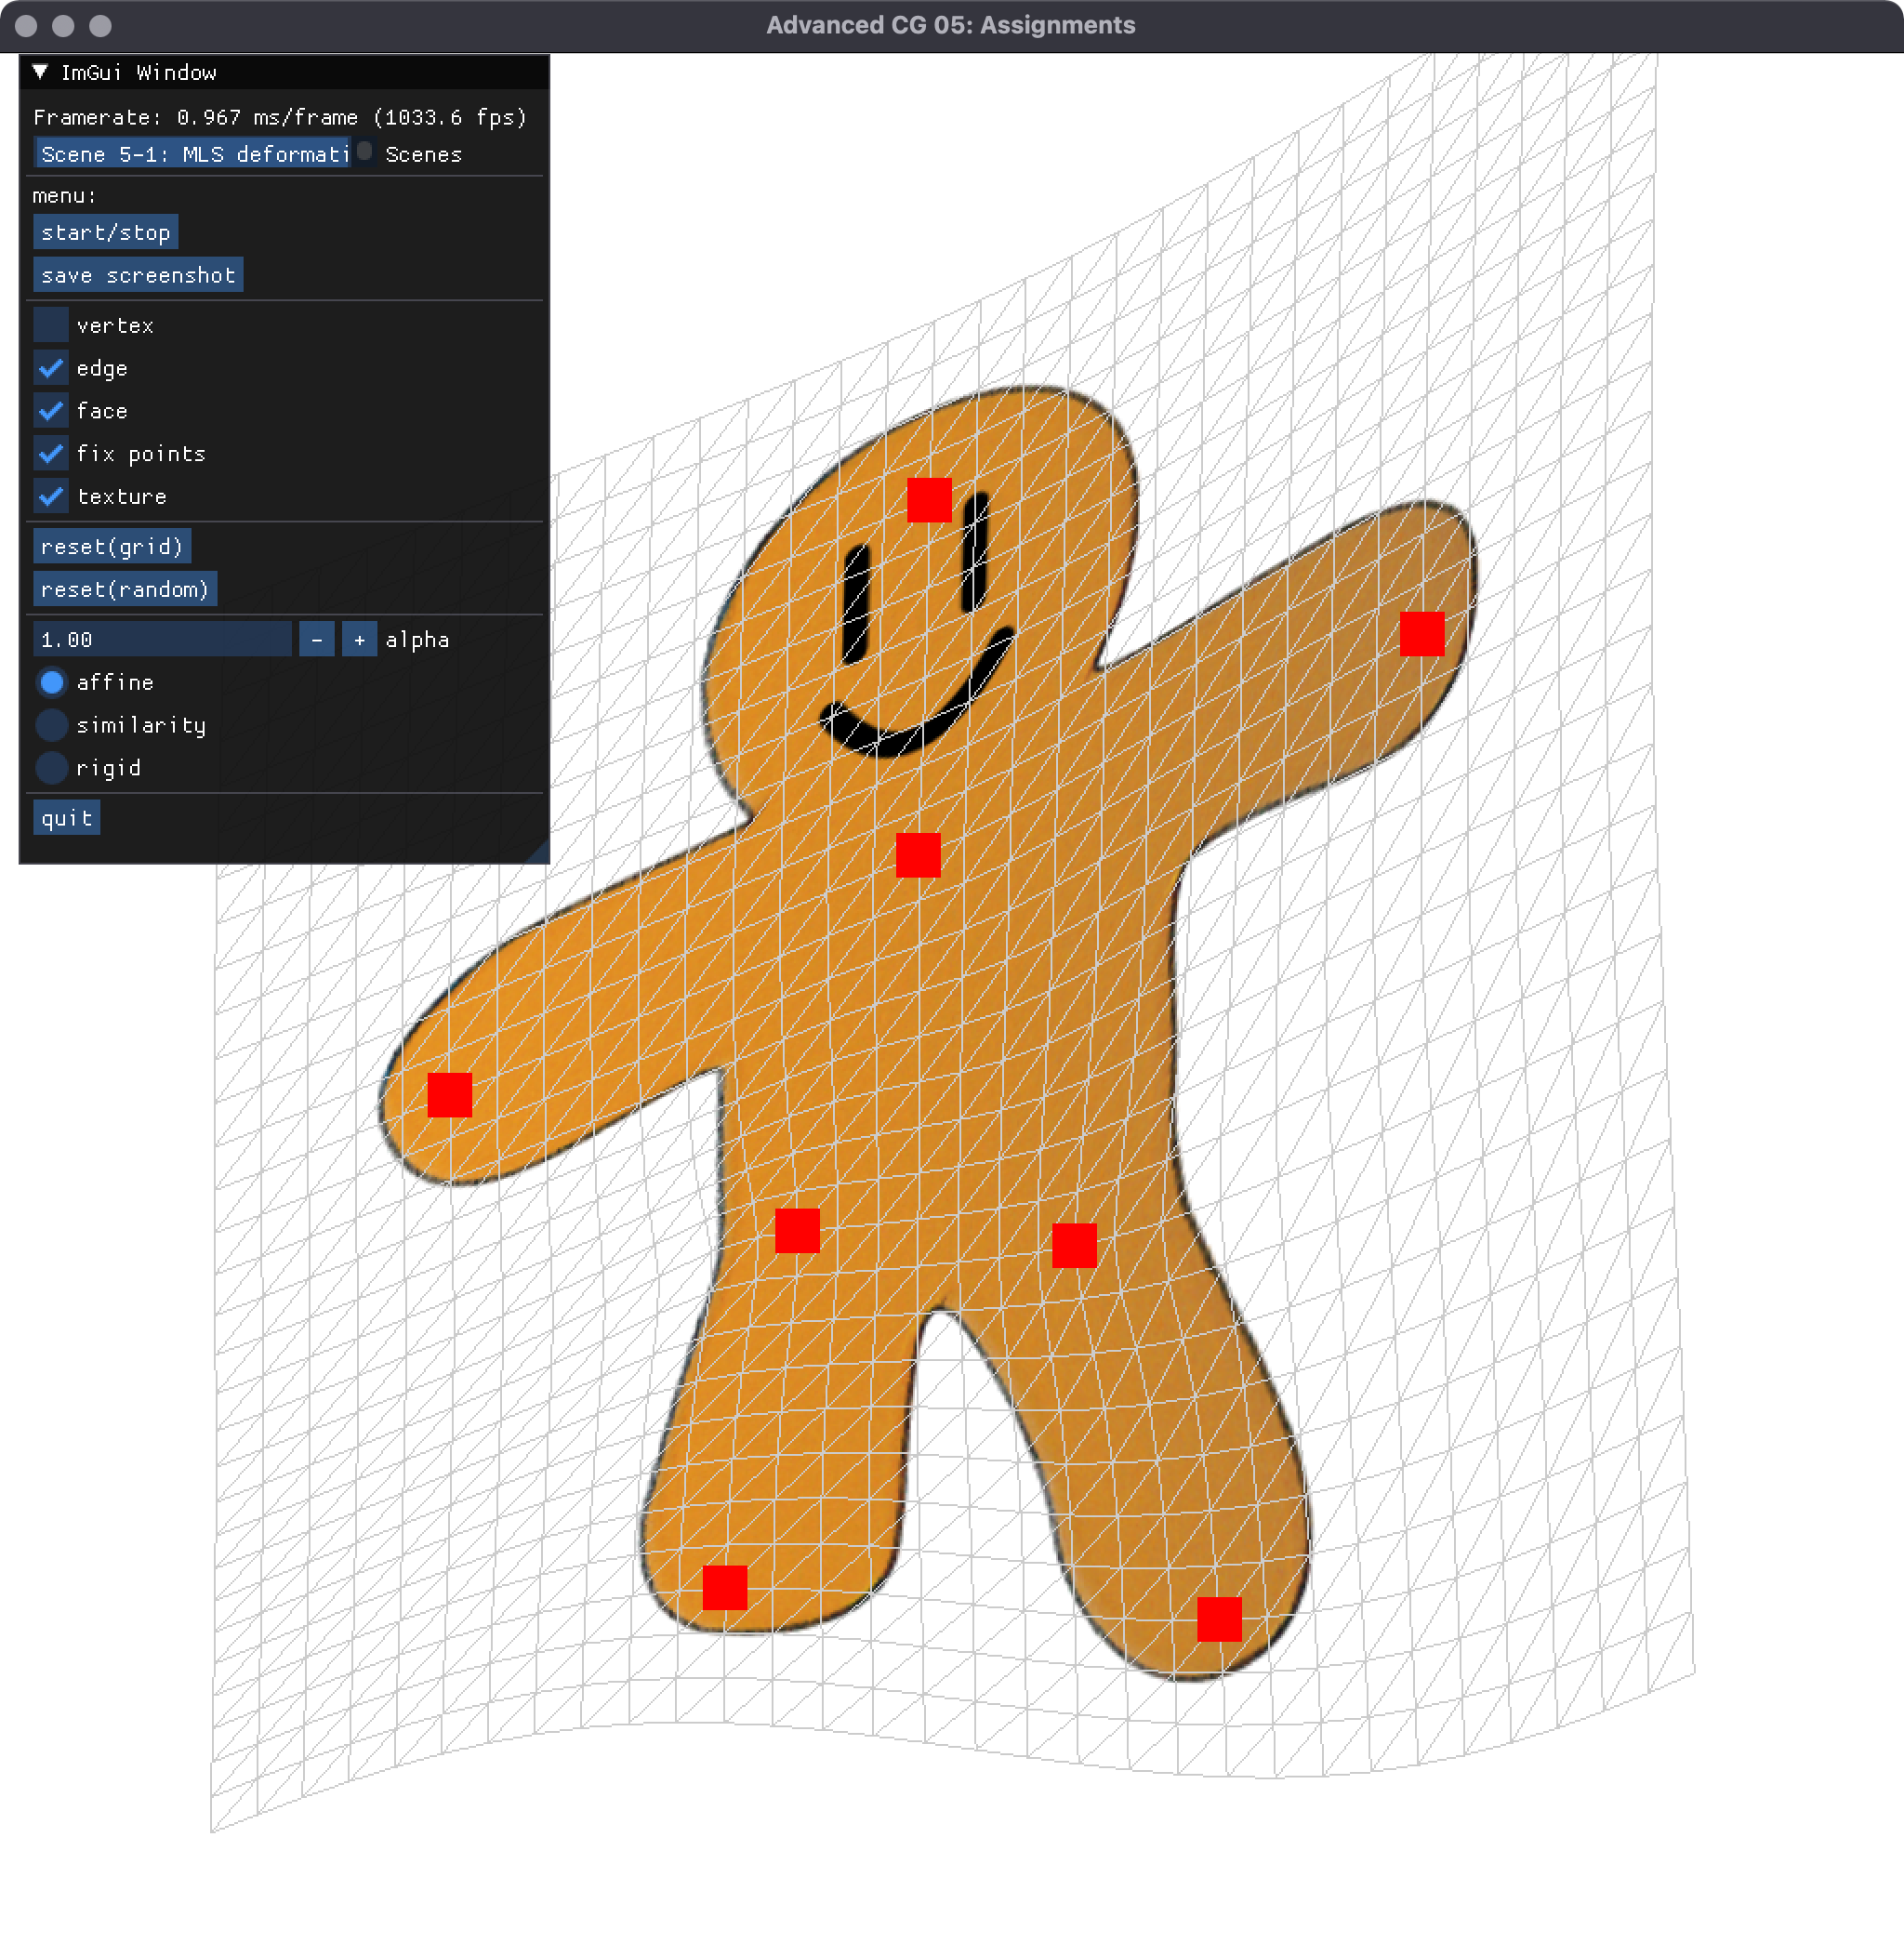
\includegraphics[width=6cm]{./img/affine.png}
  \caption{Affine Deformationの実行結果}

  \vspace{5mm}

  \centering
  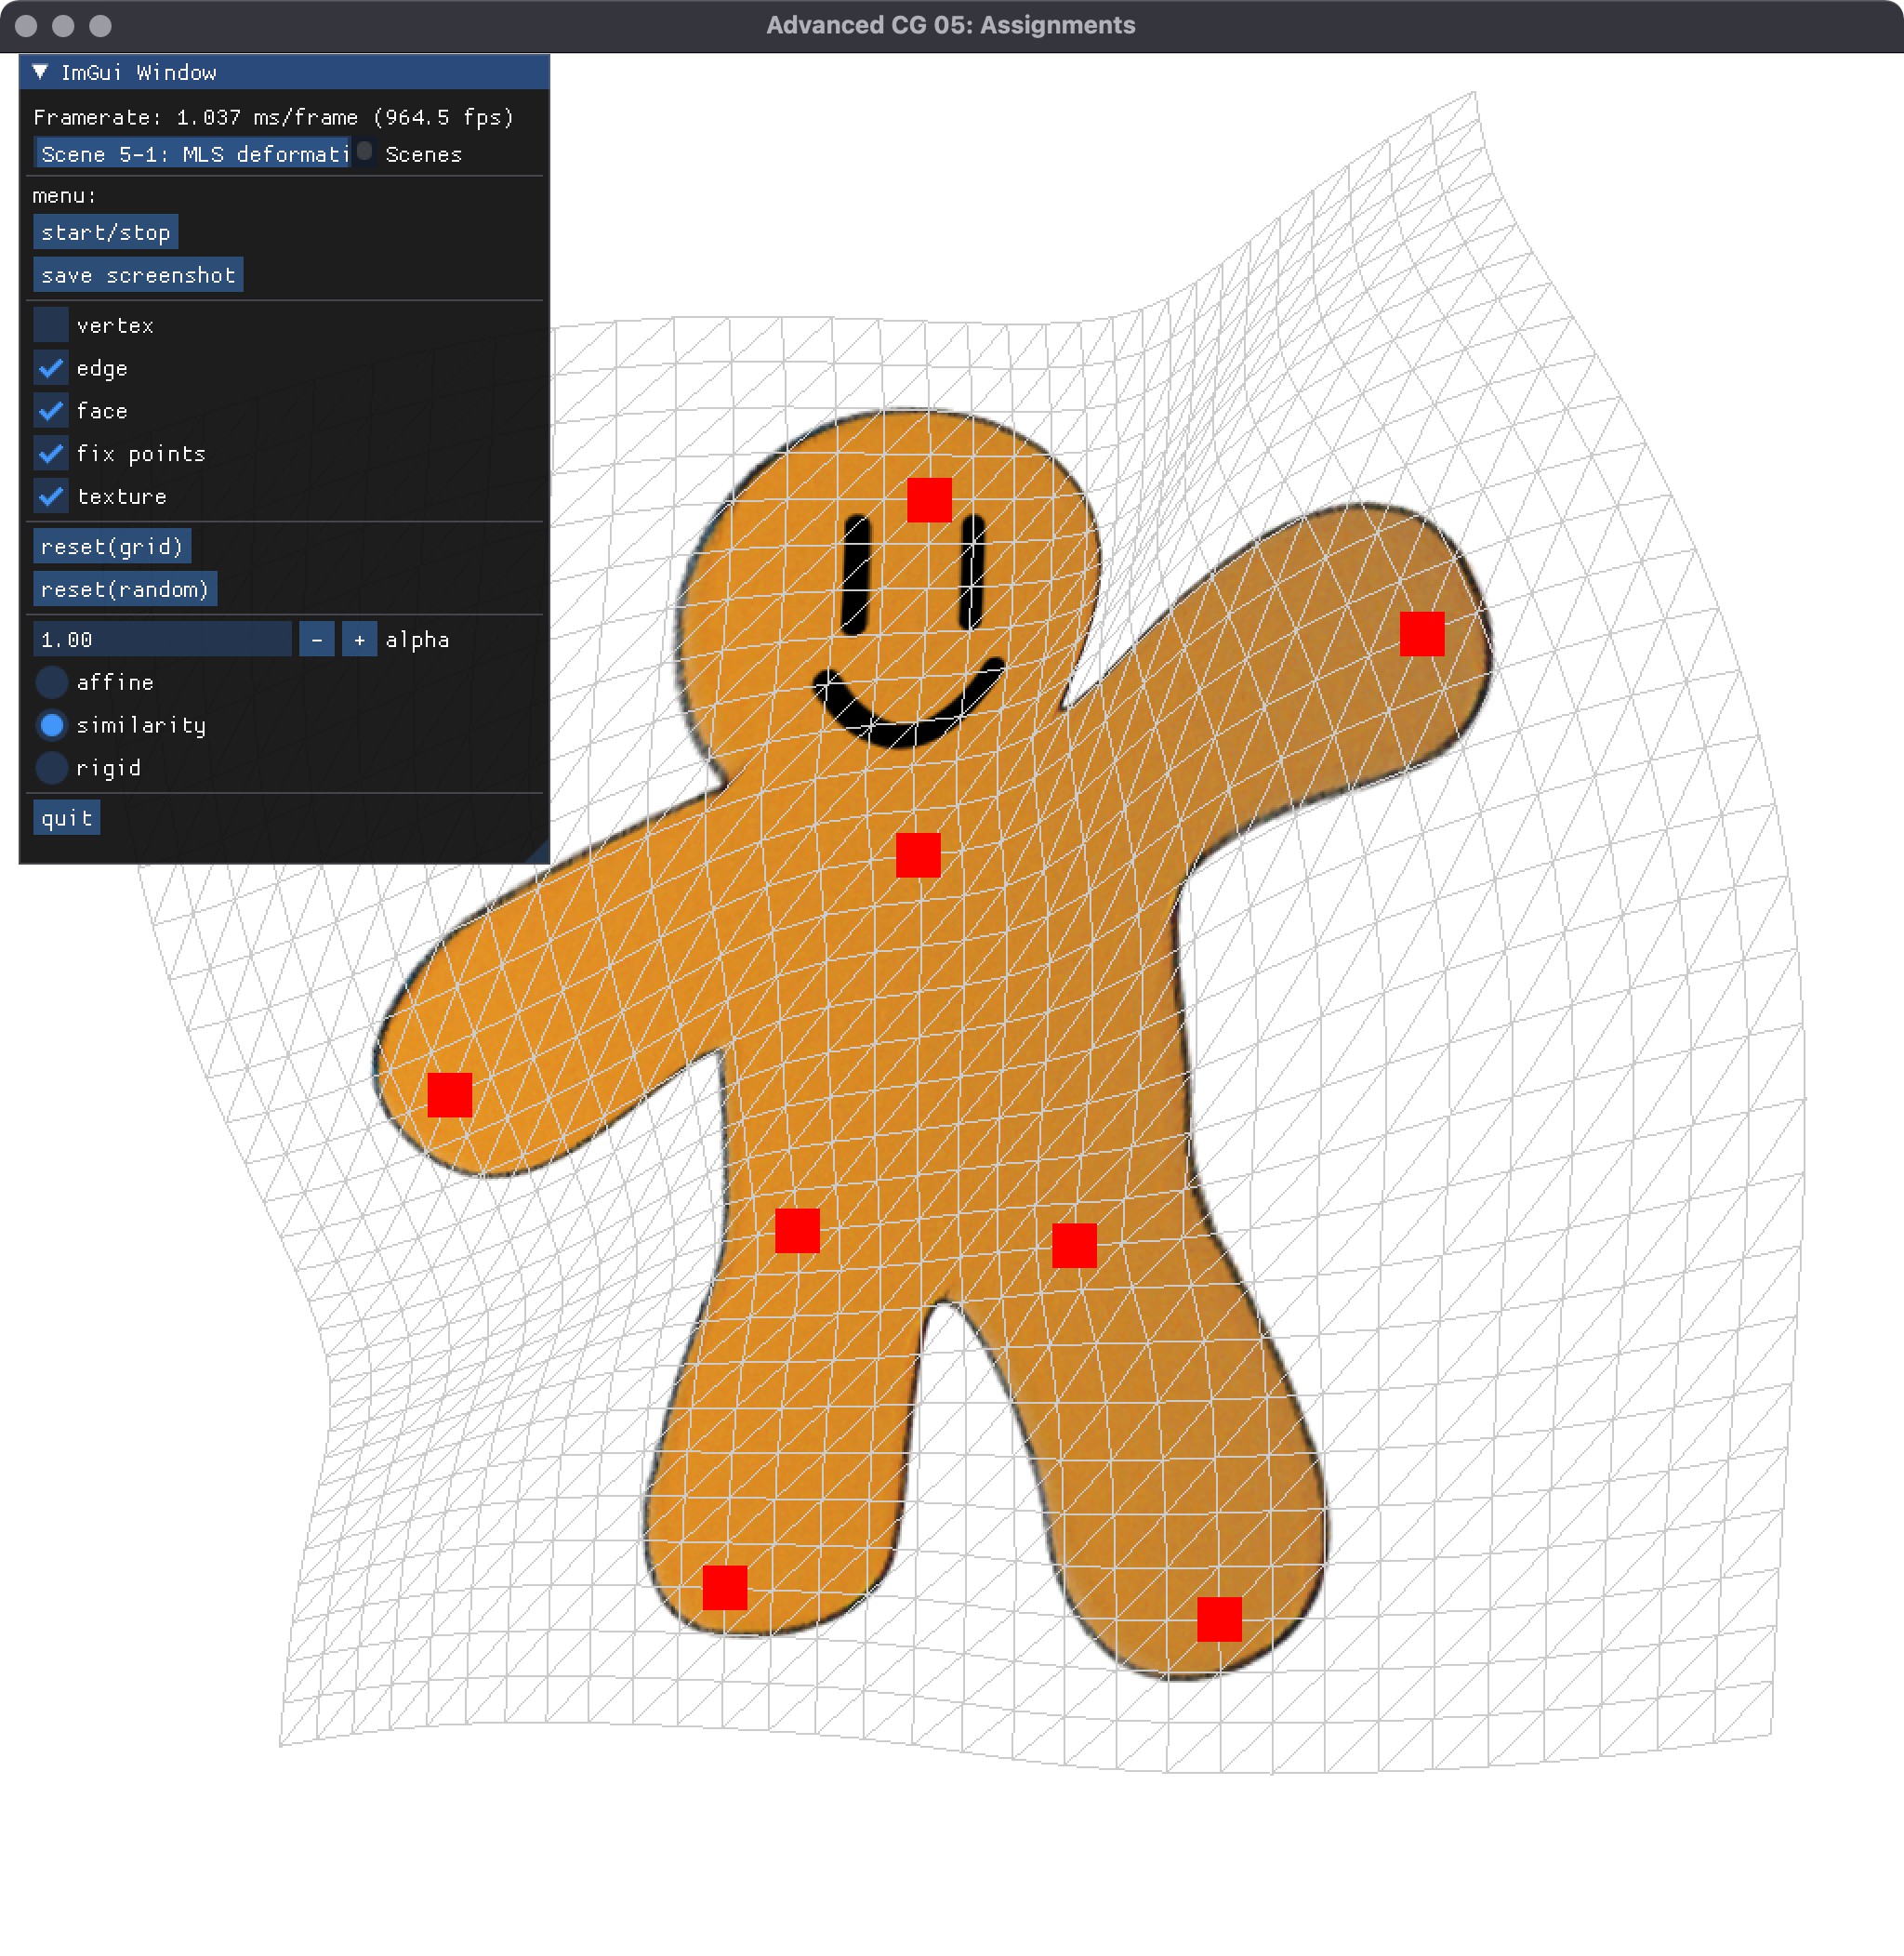
\includegraphics[width=6cm]{./img/similarity.png}
  \caption{Similarity Deformationの実行結果}

  \vspace{5mm}

  \centering
  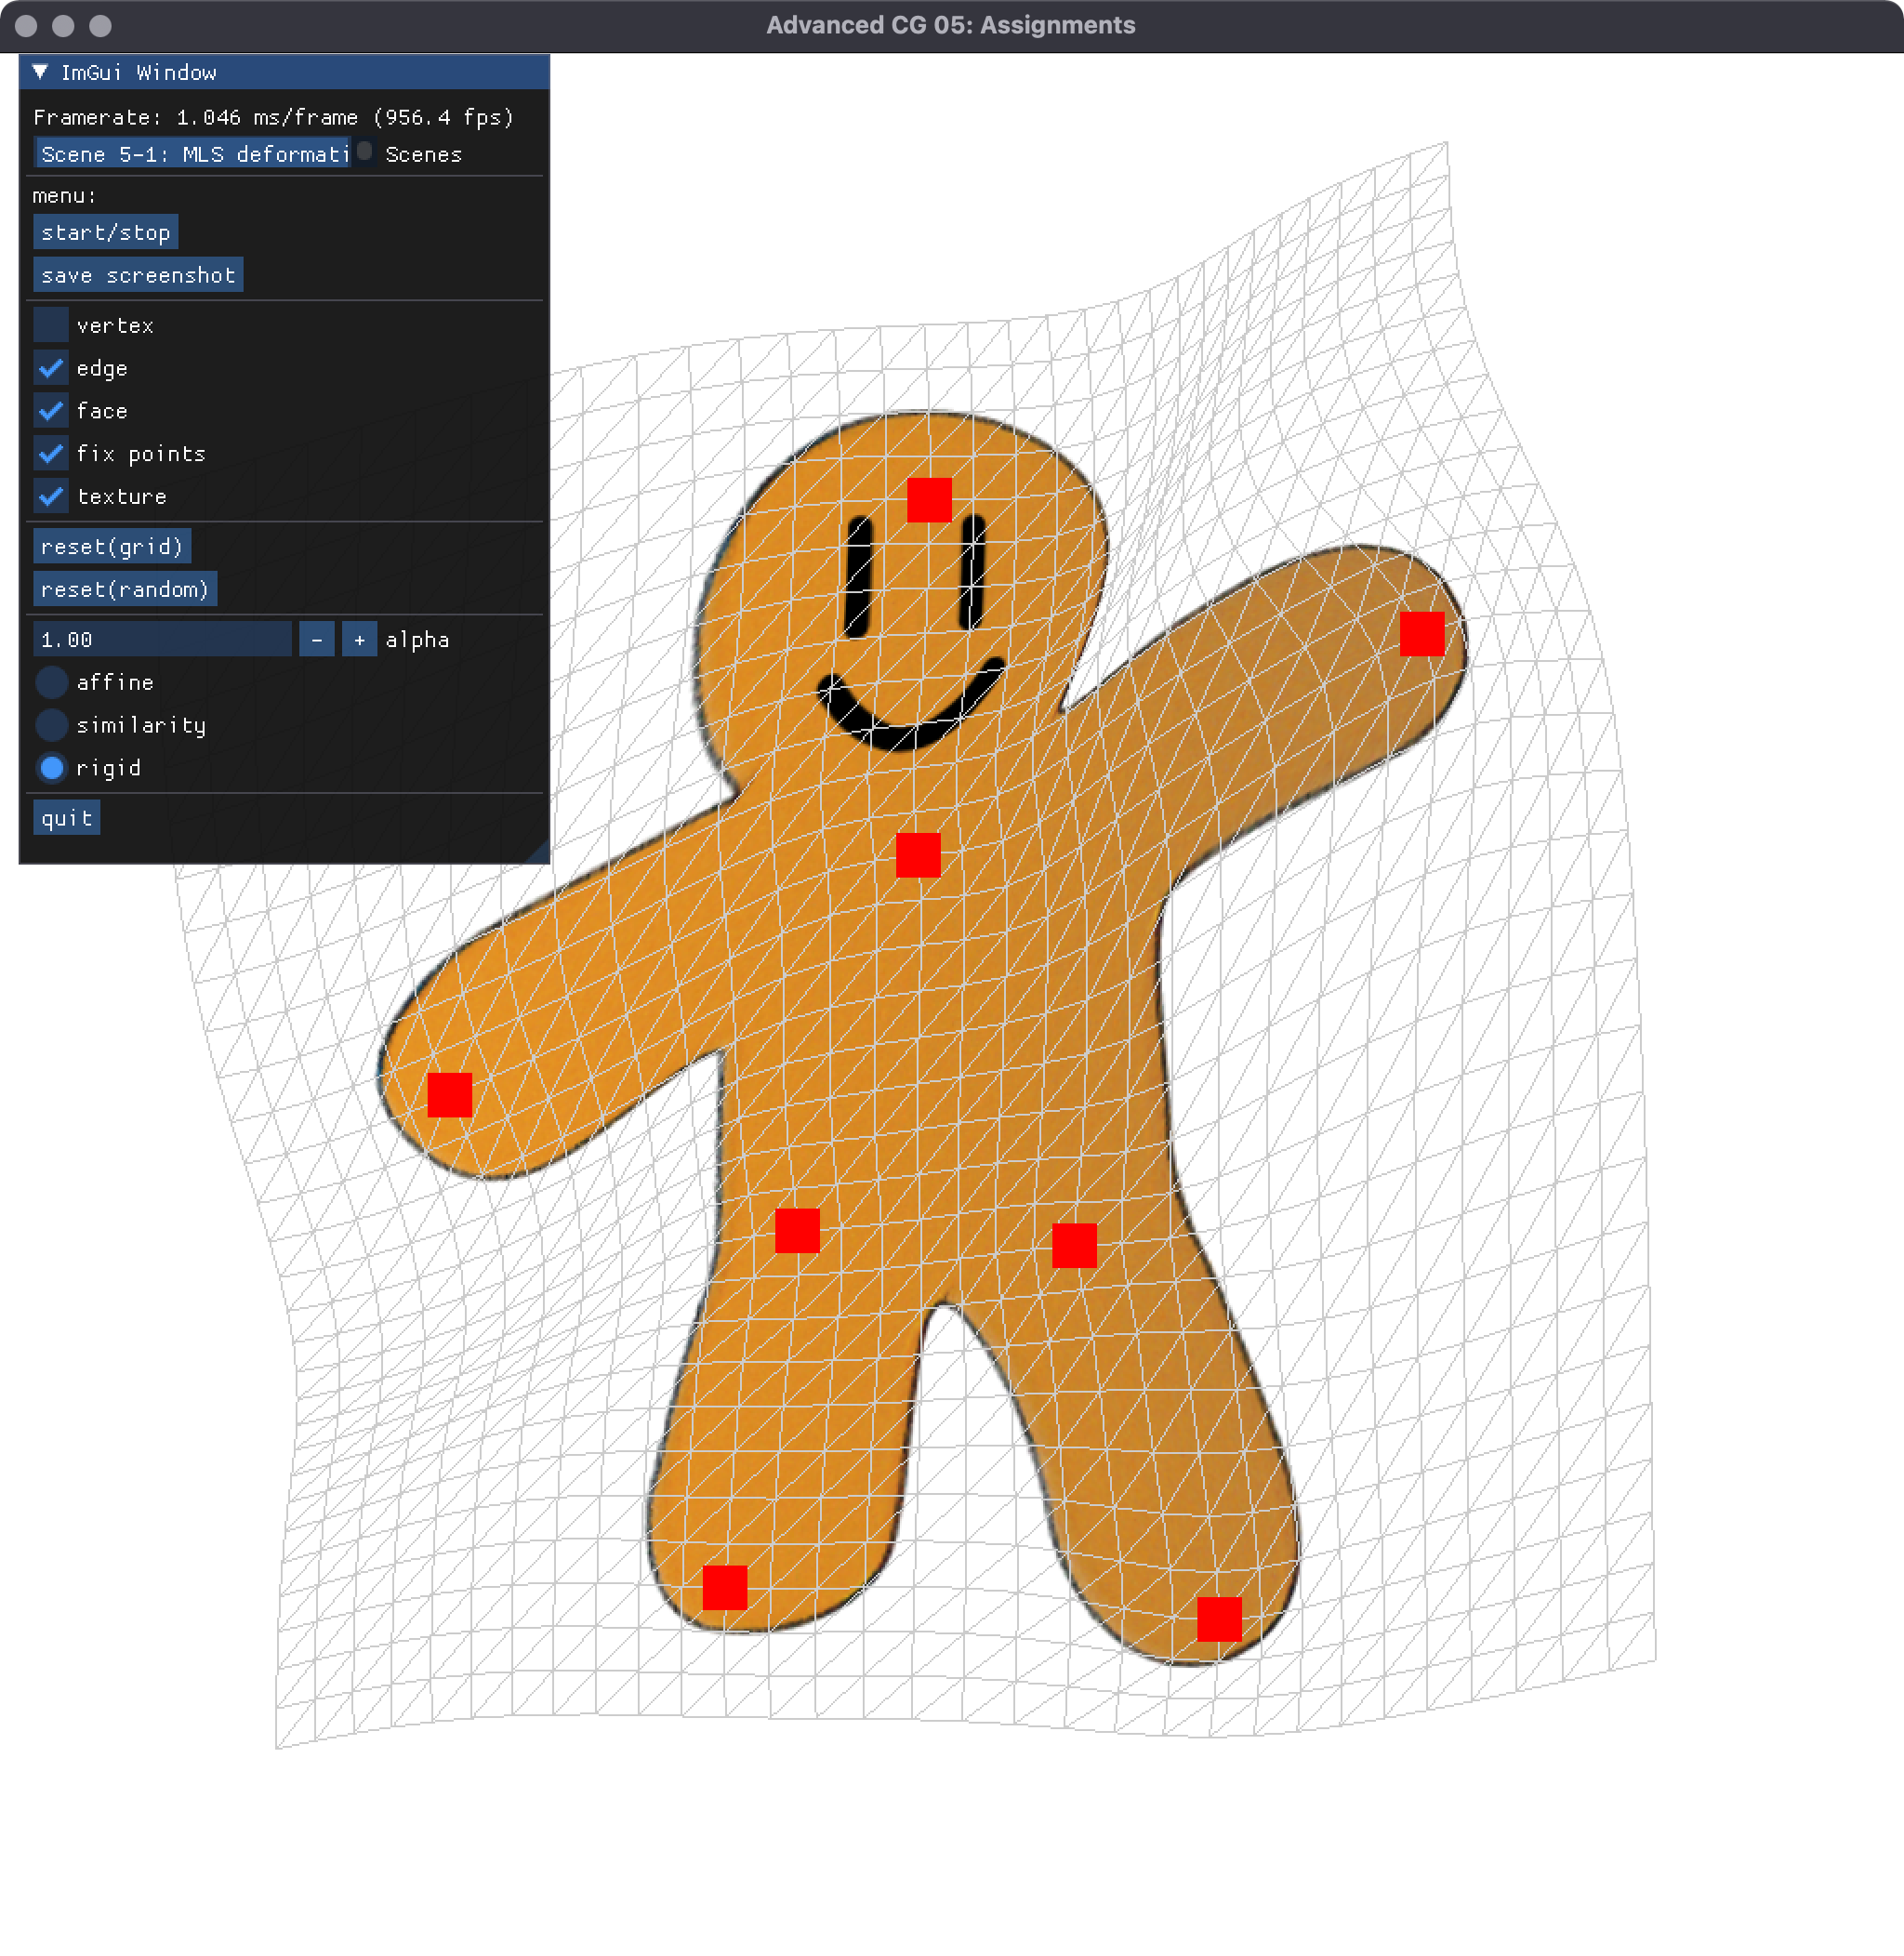
\includegraphics[width=6cm]{./img/rigid.png}
  \caption{Rigid Deformationの実行結果}
\end{figure}

\end{document}